\documentclass{article}

\usepackage{amsmath,amssymb,bm}
\usepackage{graphicx}
\usepackage{natbib}
\usepackage[latin1]{inputenc}
%\usepackage[english,french]{babel}
%\usepackage{lineno}
\usepackage{tikz}
\setlength{\doublerulesep}{\arrayrulewidth}
\usepackage{setspace}

%%%% Comment these two lines to get journal format %%%
%\renewcommand{\baselinestretch}{1.8} % the double line spacing
%\usepackage{endfloat}
%%%%

\usepackage{verbatim}
%\usepackage[x11names, rgb]{xcolor}
%\usepackage{tikz}

\newcommand{\ie}{i.e.\ }
\newcommand{\eg}{e.g.\ }

%\linenumbers
\textwidth=17cm
\marginparwidth=0cm
\hoffset=-2cm

\begin{document}
\begin{center}
\Large Ranging experiments\\ \normalsize
Martin W.\ Pedersen, Kevin Weng\\
Compiled: \today  
\end{center}

\textbf{Abstract}\\
Questions: 
\begin{enumerate}
\item Where on the vertical axis should receivers be placed to get the best detection efficiency?
\item At what depth are fish easiest to detect?
\item Can detection efficiency at one depth predict efficiency at other depths?
\end{enumerate}

 
\newpage
\section{Introduction} \label{sec:introduction} 

\section{Methods}
\label{sec:methods}

Six transmitters were deployed at two locations and three different heights relative to the bottom (3 m, 30 m, and 60 m off the sea floor). Three receivers were deployed at a different location but at the same three heights as the transmitters. Data received from the receivers are structured in a three-dimensional array $y_t(i,j)$, where $t$ is time, $i\in \{1,\ldots,6\}$ refers to transmitter number and $j\in \{1,2,3\}$ refers to receiver number.

\subsection{Information extrapolation}

Can information collected with one receiver-transmitter combination be used to infer detection efficiency at other receiver-transmitter combinations? To answer this question we construct a simple linear regression

\begin{equation}
  y_t(i,j) = \mu(i,j) + \theta[y_t(k,l)-\mu(k,l)] + e_t,
\label{eq:eff1}
\end{equation}
where $\mu(i,j) = \frac{1}{T}\sum_t y_t(i,j)$, $e_t \sim N(0,\sigma^2)$, and $\theta$ is a proportionality parameter. This model was fitted to the following scenarios:

\begin{itemize}
\item For a given transmitter how do the data vary for different receivers (at different depths)? Hourly intervals.
\item For a given receiver how do the data vary for different transmitters? Longer intervals.
\end{itemize}

\section{Results}
\label{sec:results}

Collected pinger data from the eighteen different combinations transmitters and receiver are binned into hourly intervals (Figure~\ref{fig:detectionpercentage}).

\begin{figure}
  \begin{center}
    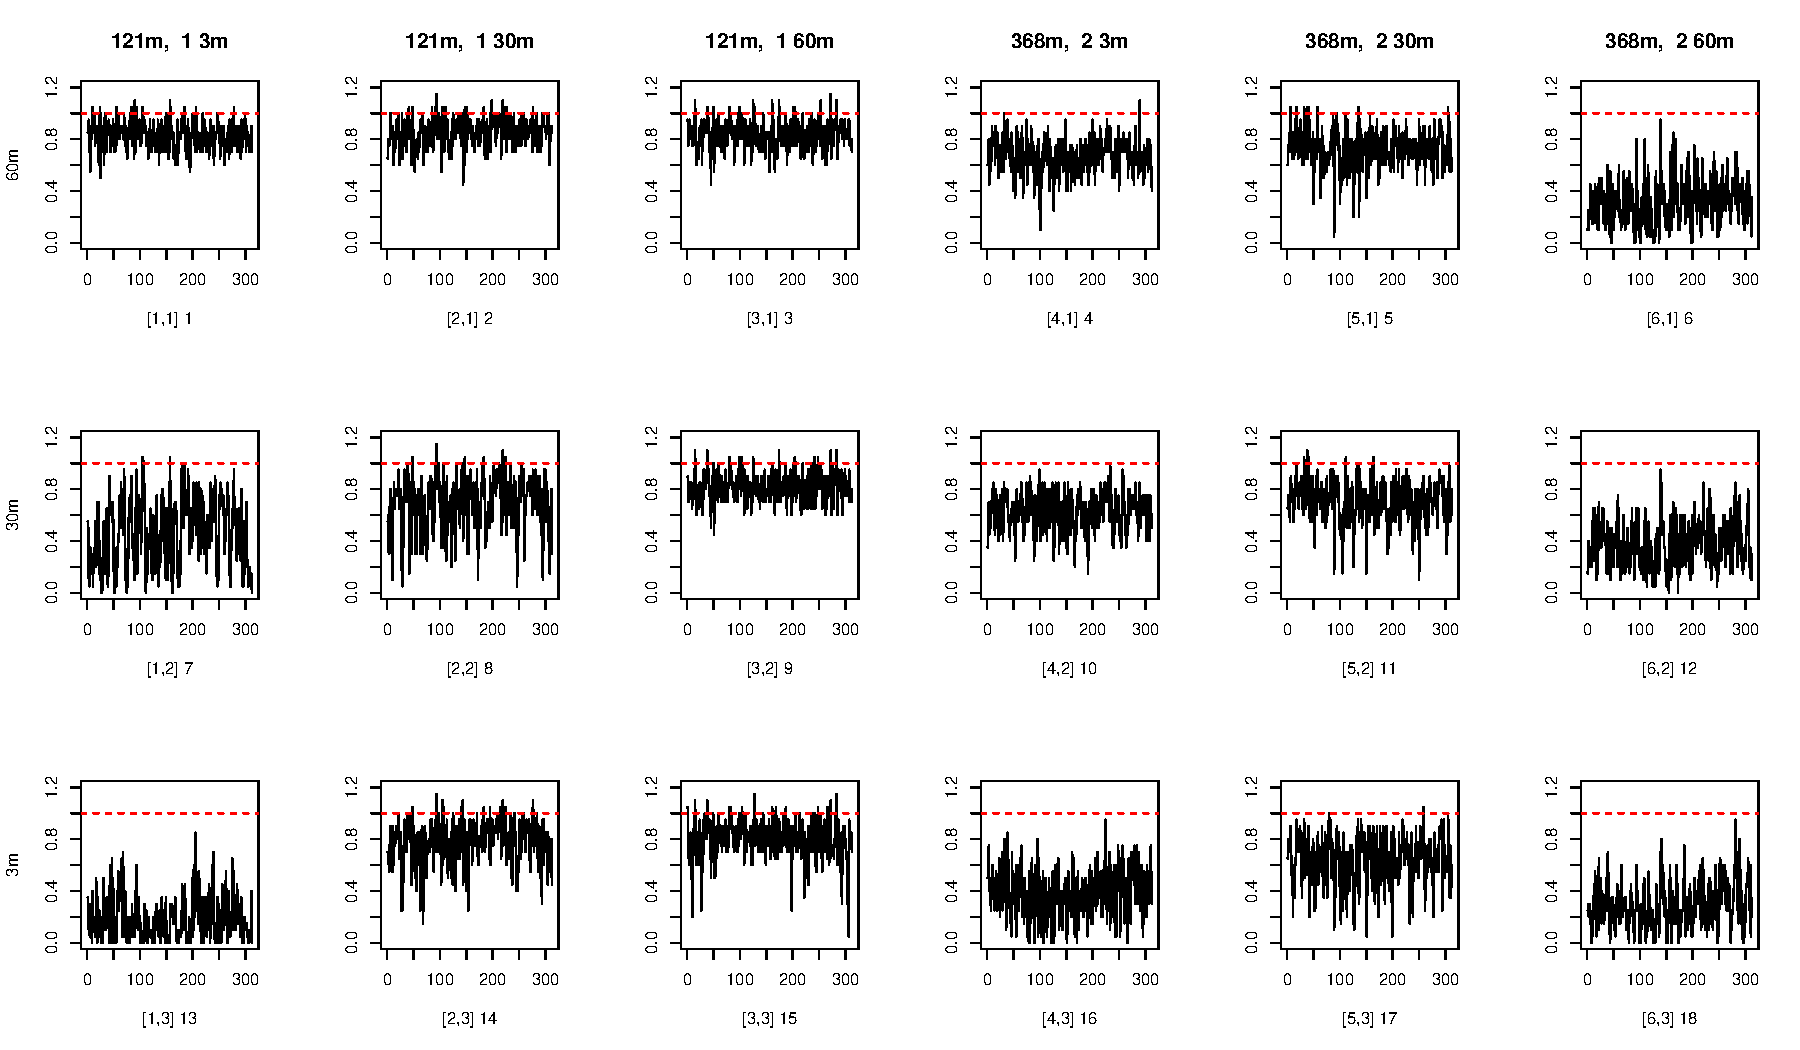
\includegraphics[trim=0cm 0cm 0cm 0cm,clip,angle=0,width=1\textwidth]{detectionpercentage.pdf}
  \end{center}
  \caption{Proportion of expected pings received at different depths for receiver and transmitter.}
\label{fig:detectionpercentage}
\end{figure}

\subsection{Fixed transmitter, different receiver}

The linear model (\ref{eq:eff1}) was fitted to combinations of data. Estimates of $\theta$ are shown in Table~\ref{tab:coeff}, $R^2$ and residual standard errors are shown in Tables~\ref{tab:rsquare} and \ref{tab:resse}. A poor fit 

% latex.default(coeff, label = "tab:coeff", caption = "Values of $\\theta$ for fit of different transmitter combinations.") 
%
\begin{table}[!tbp]
\caption{Values of $\theta$ for fit of different transmitter combinations.\label{tab:coeff}} 
\begin{center}
\begin{tabular}{lrrrrrr}
\hline\hline
\multicolumn{1}{l}{coeff}&\multicolumn{1}{c}{t1 3 m}&\multicolumn{1}{c}{t1 30 m}&\multicolumn{1}{c}{t1 60 m}&\multicolumn{1}{c}{t2 3 m}&\multicolumn{1}{c}{t2 30 m}&\multicolumn{1}{c}{t2 60 m}\tabularnewline
\hline
30~60&$0.611$&$0.840$&$0.836$&$0.615$&$0.735$&$0.547$\tabularnewline
3~60&$0.273$&$0.866$&$0.721$&$0.380$&$0.666$&$0.420$\tabularnewline
3~30&$0.099$&$0.580$&$0.991$&$0.376$&$0.653$&$0.495$\tabularnewline
\hline
\end{tabular}
\end{center}
\end{table}


% latex.default(rsquare, label = "tab:rsquare", caption = "Values of $R^2$ for fit of different transmitter combinations.") 
%
\begin{table}[!tbp]
\caption{Values of $R^2$ for fit of different transmitter combinations.\label{tab:rsquare}} 
\begin{center}
\begin{tabular}{lrrrrrr}
\hline\hline
\multicolumn{1}{l}{rsquare}&\multicolumn{1}{c}{t1 3 m}&\multicolumn{1}{c}{t1 30 m}&\multicolumn{1}{c}{t1 60 m}&\multicolumn{1}{c}{t2 3 m}&\multicolumn{1}{c}{t2 30 m}&\multicolumn{1}{c}{t2 60 m}\tabularnewline
\hline
30~60&$0.069$&$0.203$&$0.743$&$0.356$&$0.518$&$0.333$\tabularnewline
3~60&$0.043$&$0.321$&$0.305$&$0.084$&$0.295$&$0.225$\tabularnewline
3~30&$0.030$&$0.502$&$0.543$&$0.087$&$0.297$&$0.280$\tabularnewline
\hline
\end{tabular}
\end{center}
\end{table}


% latex.default(resse, label = "tab:resse", caption = "Values of residual standard error for fit of different transmitter combinations.") 
%
\begin{table}[!tbp]
\caption{Values of residual standard error for fit of different transmitter combinations.\label{tab:resse}} 
\begin{center}
\begin{tabular}{lrrrrrr}
\hline\hline
\multicolumn{1}{l}{resse}&\multicolumn{1}{c}{t1 3 m}&\multicolumn{1}{c}{t1 30 m}&\multicolumn{1}{c}{t1 60 m}&\multicolumn{1}{c}{t2 3 m}&\multicolumn{1}{c}{t2 30 m}&\multicolumn{1}{c}{t2 60 m}\tabularnewline
\hline
30~60&$0.266$&$0.198$&$0.056$&$0.126$&$0.123$&$0.148$\tabularnewline
3~60&$0.152$&$0.150$&$0.125$&$0.191$&$0.178$&$0.150$\tabularnewline
3~30&$0.153$&$0.128$&$0.101$&$0.190$&$0.178$&$0.144$\tabularnewline
\hline
\end{tabular}
\end{center}
\end{table}


% latex.default(round(pvals, digits = 3), label = "tab:pvals",      caption = "Testing for difference in means between transmitters (normality assumed).",      file = "pvals.tex") 
%
\begin{table}[!tbp]
\caption{Testing for difference in means between transmitters (normality assumed).\label{tab:pvals}} 
\begin{center}
\begin{tabular}{lrrrrrr}
\hline\hline
\multicolumn{1}{l}{round}&\multicolumn{1}{c}{3,30}&\multicolumn{1}{c}{3,60}&\multicolumn{1}{c}{30,60}&\multicolumn{1}{c}{3,30}&\multicolumn{1}{c}{3,60}&\multicolumn{1}{c}{30,60}\tabularnewline
\hline
r 60 m&$0.006$&$0.174$&$0.049$&$0$&$0$&$0$\tabularnewline
r 30 m&$0.000$&$0.000$&$0.000$&$0$&$0$&$0$\tabularnewline
r 3 m&$0.000$&$0.000$&$0.128$&$0$&$0$&$0$\tabularnewline
\hline
\end{tabular}
\end{center}
\end{table}


% latex.default(round(pvals2, digits = 3), label = "tab:pvals2",      caption = "Testing for difference in means between transmitters (non-parametric, Mann-whitney test).",      file = "pvals2.tex") 
%
\begin{table}[!tbp]
\caption{Testing for difference in means between transmitters (non-parametric, Mann-whitney test).\label{tab:pvals2}} 
\begin{center}
\begin{tabular}{lrrrrrr}
\hline\hline
\multicolumn{1}{l}{round}&\multicolumn{1}{c}{3,30}&\multicolumn{1}{c}{3,60}&\multicolumn{1}{c}{30,60}&\multicolumn{1}{c}{3,30}&\multicolumn{1}{c}{3,60}&\multicolumn{1}{c}{30,60}\tabularnewline
\hline
r 60 m&$0.003$&$0.181$&$0.084$&$0$&$0$&$0$\tabularnewline
r 30 m&$0.000$&$0.000$&$0.000$&$0$&$0$&$0$\tabularnewline
r 3 m&$0.000$&$0.000$&$0.244$&$0$&$0$&$0$\tabularnewline
\hline
\end{tabular}
\end{center}
\end{table}



\section{Discussion}
\label{sec:discussion}


\bibliographystyle{elsarticle-harv}
\bibliography{/home/mwp/work/refs/refs}

\end{document}
